% Multiple Choice Question 9 to 11 (3 questions)

\textbf{See the instruction for questions \inteval{\value{question}+1} to \inteval{\value{question}+3}.} 

\begin{center}
    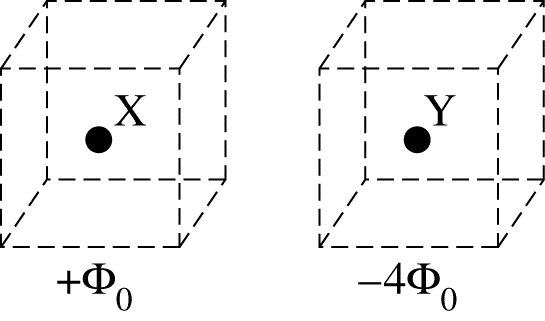
\includegraphics[scale=0.3]{images/img-006-010.png}
\end{center}

The figure above shows two charged spherical conductors, X and Y, which are equal in size. When each conductor is isolated and surrounded by a closed cubical surface, the total electric flux through the surfaces is $+\Phi_{0}$ for conductor $X$ and $-4 \Phi_{0}$ for conductor Y.

% Multiple Choice Question 9
\begin{center}
    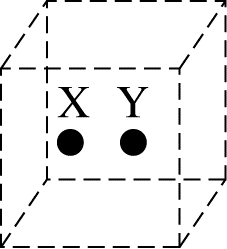
\includegraphics[scale=0.3]{images/img-006-011.png}
\end{center}

\begin{questions}
\setcounter{question}{8}

\question
Conductor Y is brought into contact with conductor X and then separated. If the separation is small so that both conductors are inside the same closed cubical surface, as shown above, what is the total electric flux through the surface?

\begin{choices}
    \choice $-3 \Phi_{0}$
    \choice $-\dfrac{5}{2} \Phi_{0}$
    \choice $-\dfrac{3}{2} \Phi_{0}$
    \choice $\dfrac{5}{2} \Phi_{0}$
    \choice It cannot be determined without knowing the distance separating the two conductors and the individual charges on each.
\end{choices}
\end{questions}

% Multiple Choice Question 10
\begin{center}
    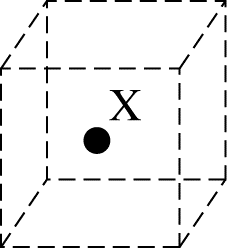
\includegraphics[scale=0.3]{images/img-006-012.png}
\end{center}

\begin{questions}
\setcounter{question}{9}
\question
After being brought into contact with conductor X, conductor Y is moved a very large distance away from conductor X. What is the total electric flux through a closed cubical surface surrounding conductor X, as shown above?

\begin{oneparchoices}
    \choice $-3 \Phi_{0}$
    \choice $-\dfrac{3}{2} \Phi_{0}$
    \choice $ \dfrac{1}{2} \Phi_{0}$
    \choice $\Phi_{0}$
    \choice $ \dfrac{3}{2} \Phi_{0}$
\end{oneparchoices}
\end{questions}

% Multiple Choice Question 11
\begin{center}
    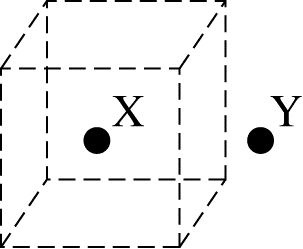
\includegraphics[scale=0.3]{images/img-006-013.png}
\end{center}

\begin{questions}
\setcounter{question}{10}
\question
Conductor Y is then moved closer to conductor X until it is just outside a closed cubical surface containing conductor X, as shown in the figure above. How would the total electric flux through the cubical surface change as conductor Y is moving?

\begin{choices}
    \choice  It would increase.
    \choice  It would decrease.
    \choice  It would change sign.
    \choice  It would remain constant, with the flux through each side of the surface also remaining constant.
    \choice  It would remain constant, but the flux through each side of the cubical surface would change.
\end{choices}
\end{questions}
